\documentclass[12pt]{article}
\usepackage[utf8]{inputenc}
\usepackage[spanish]{babel}
\usepackage{amsmath}
\usepackage{listings}
\usepackage{color}
\usepackage{graphicx}
\usepackage{caption}
\usepackage{subcaption}
\usepackage{hyperref}
\usepackage{geometry}
\geometry{margin=1in}
\usepackage{float}

\title{Comparación entre la salida de terminal en Python y la interfaz gráfica en R Shiny}
\author{Lizbeth Estefany Caceres Tacora \\ \textit{Código: 230042}}

\date{\today}

\definecolor{codegray}{rgb}{0.5,0.5,0.5}
\definecolor{backcolor}{rgb}{0.95,0.95,0.92}

\lstdefinestyle{mystyle}{
    backgroundcolor=\color{backcolor},   
    commentstyle=\color{codegray},
    keywordstyle=\color{blue},
    numberstyle=\tiny\color{gray},
    stringstyle=\color{purple},
    basicstyle=\ttfamily\footnotesize,
    breaklines=true,
    captionpos=b,
    keepspaces=true,
    numbers=left,
    numbersep=5pt,
    showspaces=false,
    showstringspaces=false,
    showtabs=false,
    tabsize=2
}

\lstset{style=mystyle}

\begin{document}

\maketitle

\section*{Introducción}
Este informe presenta una comparación entre la ejecución de un algoritmo de Gauss-Jordan en un entorno de terminal utilizando Python y su implementación en una aplicación web interactiva mediante R Shiny. Se analizan las diferencias en la experiencia del usuario, la presentación de resultados y la interacción con la aplicación.

\section{Salida de Terminal en Python}

La implementación en Python se ejecuta en la terminal, solicitando al usuario que ingrese los coeficientes del sistema de ecuaciones y mostrando los resultados directamente en la consola.



\begin{figure}[H]
    \centering
    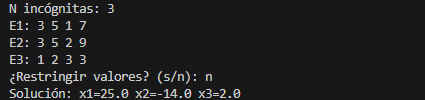
\includegraphics[width=0.8\textwidth]{salida_terminal.png}
    \caption{Captura de pantalla de la salida en terminal de Python}
    \label{fig:python_terminal}
\end{figure}

\section{Interfaz Gráfica en R Shiny}

La versión en R Shiny proporciona una interfaz gráfica donde el usuario puede ingresar la cantidad de incognitas y posterior a ello ingresar los coeficientes mediante campos numéricos y visualizar los resultados en un formato más amigable.

\begin{figure}[H]
    \centering
    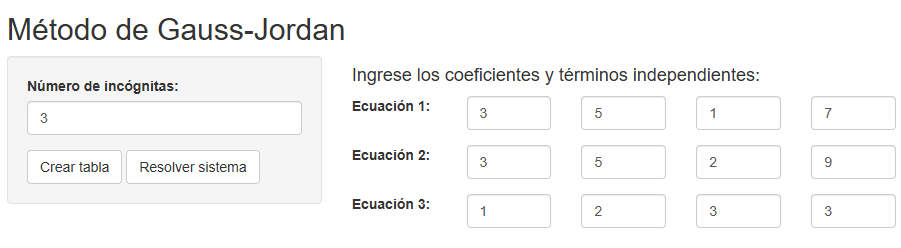
\includegraphics[width=0.8\textwidth]{r_interfaz.png}
    \caption{Interfaz gráfica de la aplicación en R Shiny}
    \label{fig:r_shiny_interface}
\end{figure}

\begin{figure}[H]
    \centering
    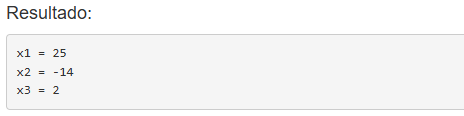
\includegraphics[width=0.8\textwidth]{salida_interfaz.png}
    \caption{Visualización de resultados en R Shiny}
    \label{fig:r_shiny_output}
\end{figure}

\section{Comparación de Experiencias}

\begin{table}[H]
\centering
\begin{tabular}{|p{5cm}|p{5cm}|}
\hline
\textbf{Python (Terminal)} & \textbf{R Shiny (Interfaz Gráfica)} \\
\hline
Interacción mediante texto en la consola & Interacción mediante campos y botones en la interfaz \\
\hline
Requiere conocimientos básicos de uso de la terminal & Intuitivo y accesible para usuarios sin experiencia técnica \\
\hline
Visualización de resultados en texto plano & Resultados presentados de forma estructurada y visualmente atractiva \\
\hline
Limitado a usuarios con acceso al entorno de desarrollo & Accesible desde cualquier navegador web \\
\hline
\end{tabular}
\caption{Comparación entre la salida de terminal en Python y la interfaz gráfica en R Shiny}
\label{tab:comparison}
\end{table}



\section{Conclusión}

La implementación del algoritmo de Gauss-Jordan en R Shiny ofrece una experiencia de usuario más interactiva y accesible en comparación con la versión en Python ejecutada en la terminal. La interfaz gráfica facilita la entrada de datos y la interpretación de los resultados, lo que puede ser especialmente beneficioso en entornos educativos o para usuarios sin experiencia en programación.

\end{document}
